\documentclass{article}
\usepackage[a4paper, margin=2.5cm]{geometry}
\usepackage{amsmath}
\usepackage{caption}
\usepackage{placeins}
\usepackage{graphicx}
\usepackage{subcaption}
\usepackage{setspace}
\usepackage{float}

%\usepackage[active,tightpage]{preview}
\usepackage{natbib}
\bibpunct{(}{)}{,}{a}{}{;} 
\usepackage{url}
\usepackage{nth}
\usepackage{authblk}
% for the d in integrals
\newcommand{\dd}{\; \mathrm{d}}
\newcommand{\tc}{\quad\quad\text{,}}
\newcommand{\tp}{\quad\quad\text{.}}
\defcitealias{HMD}{HMD}

\newcommand\ackn[1]{%
  \begingroup
  \renewcommand\thefootnote{}\footnote{#1}%
  \addtocounter{footnote}{-1}%
  \endgroup
}
\begin{document}

%\title{Macro patterns in the shape of aging}
\title{Macro shapes in the evolution of human aging}

\author[1]{Tim Riffe\thanks{riffe@demogr.mpg.de}}
\author[2,3]{Jos\'e Manuel Aburto \thanks{jmaburto@health.sdu.dk}}
\affil[1]{Max Planck Institute for Demographic Research}
\affil[2]{University of Southern Denmark}
\affil[3]{Max Planck Odense Center on the Biodemography of Aging}

\maketitle

\begin{abstract}

\end{abstract}

\section*{Extended abstract}

\doublespacing

Typically, demographers summarize the distribution of remaining
lifetimes by age using the mean, $e(a)$, i.e. life expectancy. Life expectancy at birth, $e(0)$ is one of the most widely used measures to
summarize population health. Its significant and consistent increase witnessed during the last two centuries is one of the most remarkable achievements of modern societies \citep{oeppen2002broken}. Most countries have improved in this indicator \citep{world2016world}, and the most long-lived populations have steadily increased their average length of life by 2.5 years every decade \citep{oeppen2002broken}. Nevertheless, life
expectancy is not an omnibus descriptor of time to death. There are other
useful measures of longevity the refer to the pace of aging, such as the modal or median ages at death \citep{canudas2010three}, that also summarize the distribution of mortality in a snapshot of a stationary population or else the age at death distribution of a newborn cohort under constant mortality
conditions. These indicators, however, conceal variation in lifetimes and other aspects of the age at death distribution. 

Variation in lifespans has recently arisen as an important dimension in demography and aging research. It expresses a fundamental inequality among individuals and addresses the growing interest in health inequalities, and its linkage with social behavior \citep{mackenbach2012persistence}. It has been found to be negatively associated with life expectancy levels in several countries and over millions of years of primate evolution \citep{vaupel2011life, colchero2016emergence}. As a result, demographers have responded to this need of accurate measures and have developed a battery of lifespan variability indicators \citep{van2013perturbation}, which refer to particular aspects of the shape of the distribution of mortality or the shape of aging \citep{wrycza2015quantifying}. 

In this paper, we extend on previous research by developing a set of formulas to measure other aspects of the age at death distribution from lifetables conditioned on surviving to any age, such as skewness and kurtosis, from a moment generator function. Further, we explore linkages between such indicators and the pace of aging from a macro shape framework and interpret our results on the evolution of aging context.

\subsection*{Definitions}

Remaining life expectancy conditional on survival to age $a$ is defined as
\begin{equation}
e(a) = \frac{1}{l(a)}\int_0^\infty l(a+y) \dd y \tc
\end{equation}
where $l(a)$ is lifetable survivorship to age $a$.
%Let lifespans for a given birth cohort be measured with the random variable,
%$X$, with distribution $d(X)$, identical to the $d_x$
%column of the lifetable if a radix of 1 is used. We are interested in the
%conditional density function, $f(X-a ~|~ X \ge a)$, which we denote $f(y|a)$,
% where $a$ is age attained and $y$ is remaining years of life, and which is defined as:
Define the
conditional deaths distribution
\begin{equation}
\label{eq:fya}
f(y|a) = \frac{1}{l(a)} \mu(a+y) l(a+y) \tc
\end{equation}
where $\mu(a)$ is the force of mortality at age $a$. $f(y|a)$ is interpreted as
the probability of surviving to and dying at exact age $a+y$ given survival to
age $a$.

The conditional deaths distribution can be described empirically using
quantiles, or other central measures such as the median or the mode, or perhaps more parsimoniously using its moments.
The $n^{th}$ central moment about the conditional mean of $f(y|a)$,
$\eta_n(y|a)$ is defined as:
\begin{equation}
\eta _n(y|a) =  \int_{y=0}^\infty (y-e(a))^n f(y|a) \dd y \tc
\end{equation}
where $\eta_2(y|a)$ gives the variance of remaining lifespan about $e(a)$,
$\sigma^2(y|a)$.\footnote{Compare with \citet{chiang1984life}, Chapter 10,
Equation 6.10, where the author denotes $f(y|a)$ with $Y_\alpha$.}
Survival-conditioned variance is useful information, but it can be deceptive
because lifespan variation is not symmetric around $e(a)$. The
conditional skewness function, $Skew(y|a)$ captures most such variation and can be roughly interpreted in this way. It is defined as
\begin{equation}
\label{eq:skew}
Skew(y|a) = \frac{\eta _3(y|a)}{\sigma(y|a)^3} \tc
\end{equation}
the third standardized moment. The conditional excess
kurtosis of $f(y|a)$, $Kurt(y|a)$, can be defined as
\begin{equation}
\label{eq:kurt}
Kurt(y|a) = \frac{\eta_4(y|a)}{\sigma(y|a)^4}-3 \tp
\end{equation}
The age pattern of kurtosis describes how the peakedness, or the fatness of the
tails of the remaining distribution change over age. %The coefficient of
%variation of remaining lifespan, $CV(y|a)$ is then simply
%\begin{equation}
%CV(y|a) = \frac{\sigma(y|a)}{e(a)} \tp
%\end{equation}
%$CV(y|a)$ is dimensionless and comparable over age, and its reciprocal
%can be thought of as a signal to noise ratio of one's likely remaining
% lifespan, assuming a constant mortality pattern in ages higher than $a$. Other conditional
%measures may also be devised in similar fashion, the most obvious and useful of
%which are quantiles, which we also calculate in the following empirical
% section.

\section*{Data and Methods}
All formulas are discretized to single ages
using standard demographic approximations, and these are implemented in the
\texttt{R} programming language \citep{R}. We then calculate the above measures
for each year, population, and sex in the Human Mortality Database
\citepalias{HMD}. To examine macro patterns in the central and shape measures,
we show a series of bivariate relationships.

\FloatBarrier
\section*{Preliminary Results}
% next steps, mayble show conditional on surviving to age 15, 50 and 65?
Figure \ref{fig:CV} shows the linkage between life expectancy at birth and  variation in lifespans, as measured by the coefficient of variation for 45 countries. Lighter colors refer to data before 1921, darker reds to years between 1921 and 1959, and darkest hues to the most recent period from 1960 onward. The results suggest that as populations tend to live longer, they also experience less uncertainty surrounding their eventual time of death. After 1960, there is a change in the slope and a level-off on the speed of reducing variability, as the coefficient of variation asymptotically reaches zero, the unrealistic scenario in which everybody dies at the same age.
\begin{figure}
\caption{Coefficient of variation by average length of life}
\centering
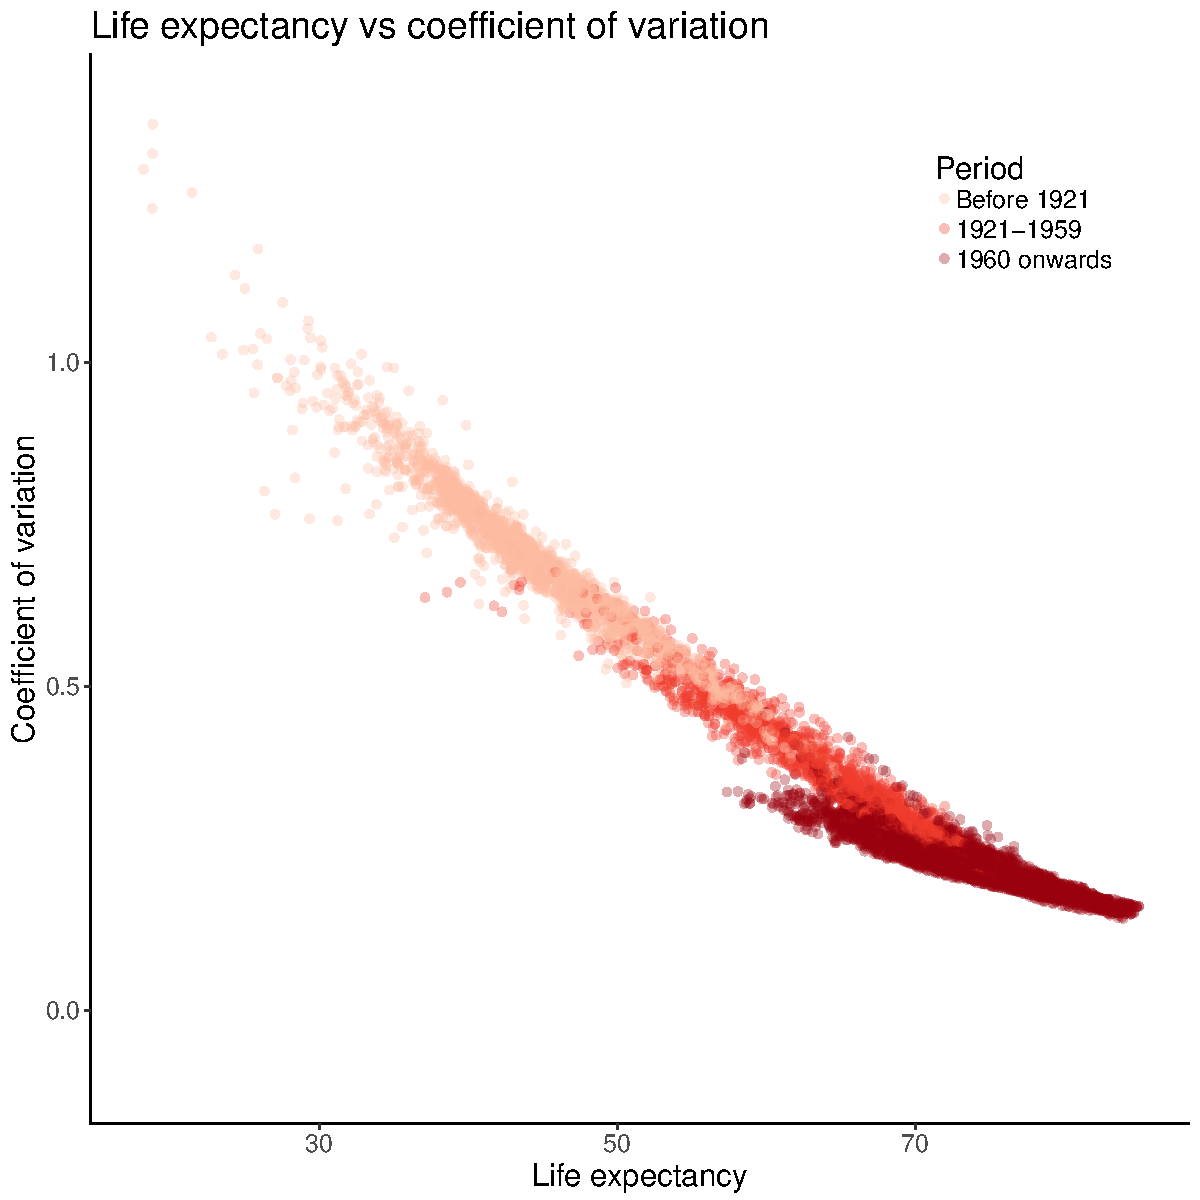
\includegraphics[width=.3\textwidth]{Figures/Figure_CV}
\label{fig:CV}
\end{figure}

Figure \ref{fig:sk&kt} shows the skewness of the age at death distribution and its linkage with the evolution of life expectancy (panel \ref{fig:sk}) and its corresponding kurtosis value (panel \ref{fig:sk}). Before 1960, the macro pattern of life expectancy with skewness suggest that as the average length of life increases over time, the distribution of mortality gets a longer left tail. However, after 1960 populations seem to have experienced a shift on the value of skewness, known in.. (insert tims concept). This might be a result of countries changing from a bimodal to a unimodal distribution. In addition, as mortality reductions are harder at young ages, improvements are gradually concentrated at older ages, which makes the right tail of the distribution longer. Similarly, as life expectancy increases, the value of kurtosis also increases. However, after 1960 similar values of life expectancy correspond to different values in kurtosis. These results suggest that over time, the tails of the distribution are getting ``fatter'', paralleling the rise in life expectancy. 

Future results: we will further compare linkages between different moments conditioned on surviving to higher ages. For example, what are the macro association between these indicators conditioned on surviving to age 15, leaving out all infant mortality and capturing 

\begin{figure}
\caption{Skewness and kurtosis at birth by average length of life}
\centering{
\begin{subfigure}{.4\textwidth}
  \centering
  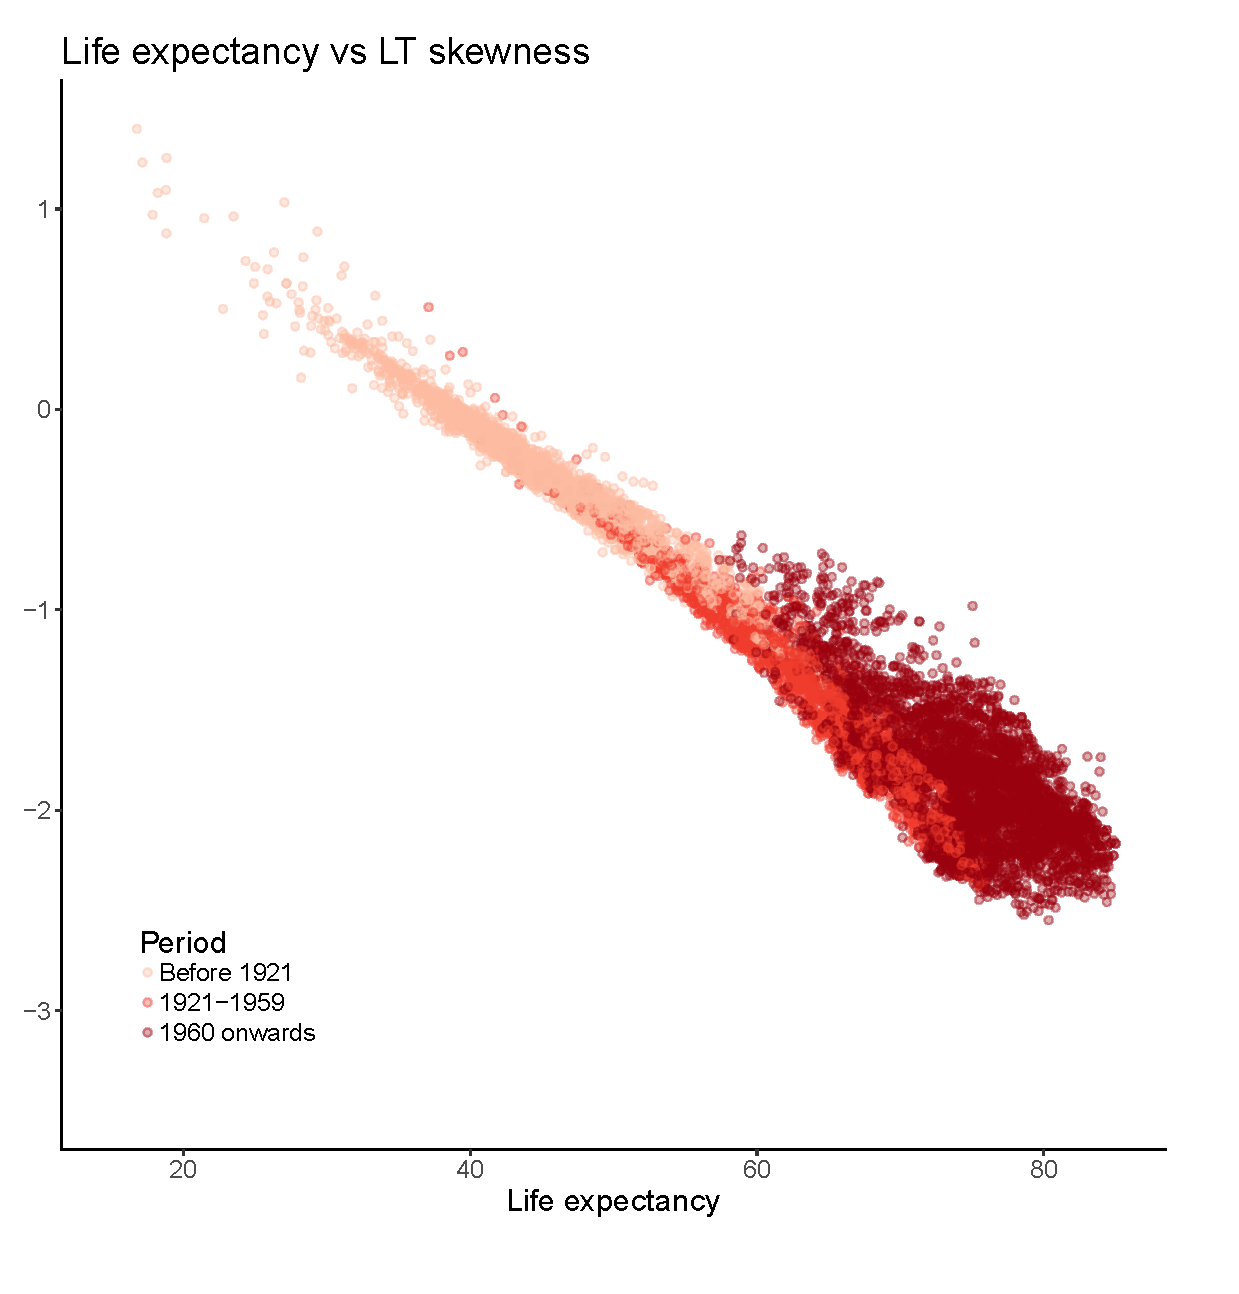
\includegraphics[width=.8\linewidth]{Figures/F2_Skew}
  \caption{Skewness vs $e(0)$}
  \label{fig:sk}
\end{subfigure}
\begin{subfigure}{.4\textwidth}
  \centering
  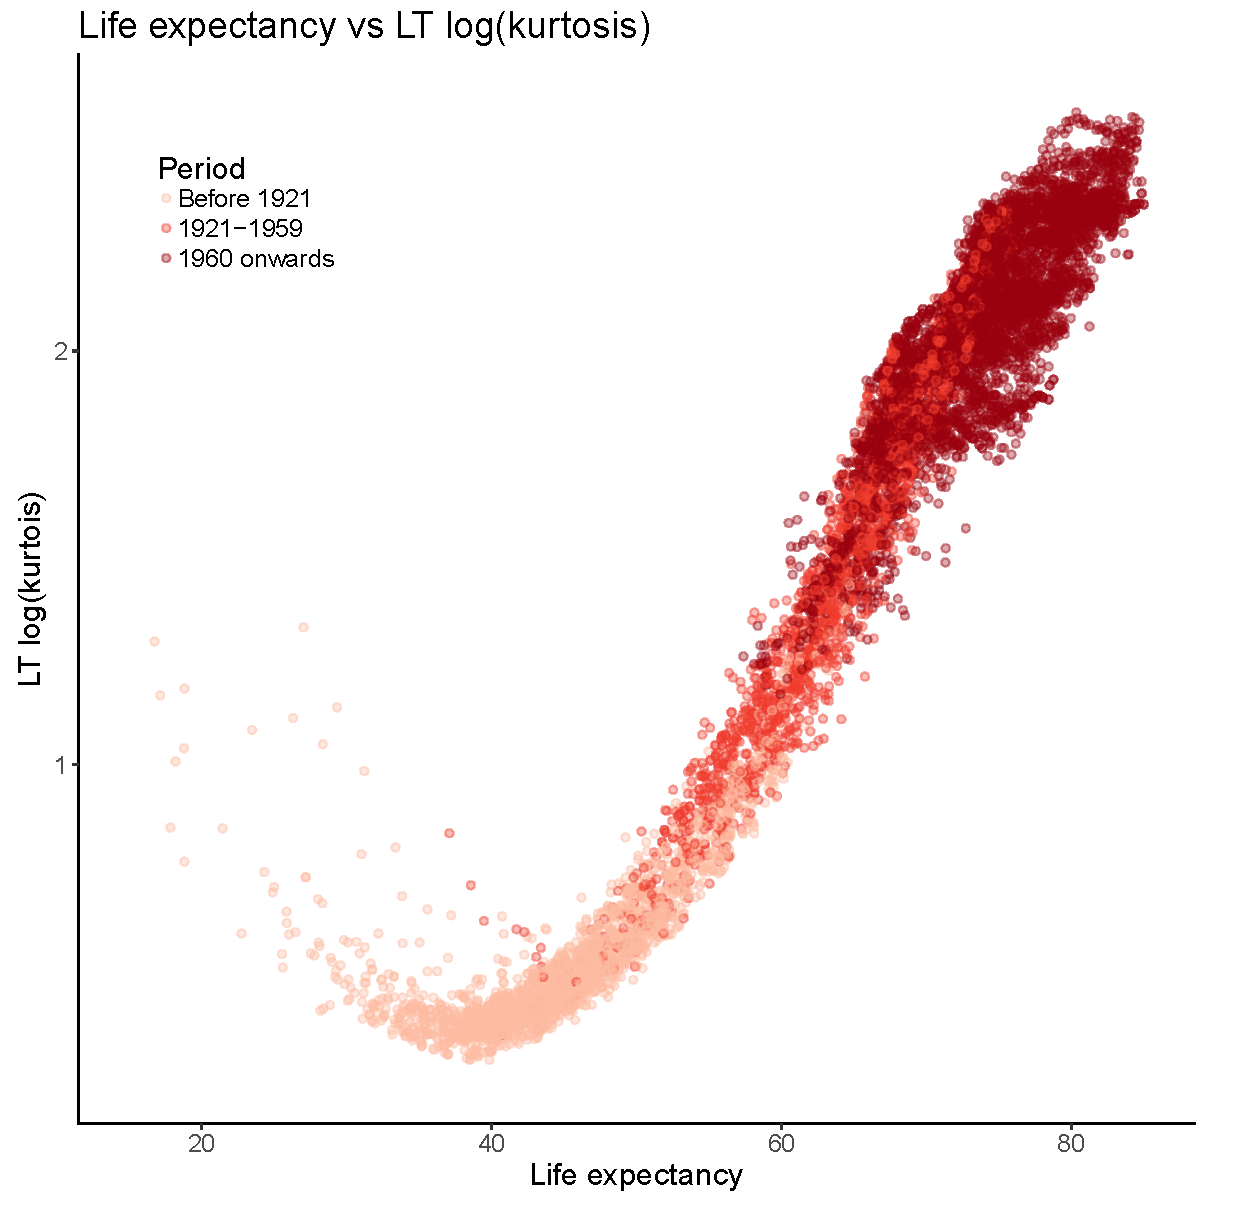
\includegraphics[width=.8\linewidth]{Figures/F1_Kurtosis}
  \caption{Kurtosis vs $e(0)$}
  \label{fig:kurt}
\end{subfigure}}
\label{fig:sk&kt}
\end{figure}

\FloatBarrier
\singlespacing
\bibliographystyle{plainnat}
  \bibliography{references} 

\end{document}
